\section{Results}
\label{sec:results}

\subsection{RQ1: Relevance --- improved, but fragile}
\label{sec:results-relevance}

On QuixBugs ($n{=}40$), \structured improves the independent fix-diff
relevance metric over \codeonly at every depth (top-5: $0.234$ vs $0.207$;
mean difference $+0.027$, 95\%~CI $[+0.016,+0.037]$; Wilcoxon $p{=}0.0001$;
higher on 31/40 problems). The tag-compatibility proxy shows the same
direction but overstates it ($0.394$ vs $0.218$, $+81\%$, against $+13\%$ on
the independent metric); we therefore treat the tag proxy as illustrative
only.

However, the gain \emph{does not replicate} on MBPP-holdout ($n{=}187$):
\codeonly $0.464$ vs \structured $0.456$ (mean difference $-0.008$, 95\%~CI
$[-0.025,+0.009]$, $p{=}0.41$). Two interpretations are compatible with one
positive and one null: (a)~the gain is benchmark-specific --- MBPP's
single-operator mutations leave a thin failure signal, and dense retrieval
already matches the near-identical buggy code, leaving no room for failure
structure to help; or (b)~the gain is simply not robust, and the
larger-sample null is the better estimate. We cannot distinguish these from
the available data, and interpretation~(a) was constructed post hoc. Either
way, the one clean positive in this study is fragile --- which sharpens
rather than weakens the questions that follow.
%% TODO(audit): report the blind human relevance audit (two annotators,
%% Cohen's kappa, per-variant human relevance rates) as the third measure.

\begin{table}
\caption{Independent relevance metric (cosine of candidate fix diff to
ground-truth fix diff), top-5 mean.}
\label{tab:relevance}
\begin{tabular}{lrrr}
\toprule
Benchmark & \codeonly & \structured & $p$ \\
\midrule
QuixBugs ($n{=}40$) & 0.207 & \textbf{0.234} & 0.0001 \\
MBPP-holdout ($n{=}187$) & 0.464 & 0.456 & 0.41 (ns) \\
\bottomrule
\end{tabular}
\end{table}

\subsection{RQ2: Conversion --- neutral to slightly negative}
\label{sec:results-conversion}

\begin{table}
\caption{Downstream repair vs.\ no-retrieval baseline (single attempt,
$k{=}2$). All differences non-significant by exact McNemar.}
\label{tab:downstream}
\begin{tabular}{llrrr}
\toprule
Benchmark & Model & base & \structured & $p$ \\
\midrule
QuixBugs & GPT-4o & 35/40 & 37/40 & ns \\
QuixBugs & GPT-4.1 & 36/40 & 35/40 & ns \\
QuixBugs & GPT-4o-mini & 33/40 & 30/40 & ns \\
HumanEvalFix & GPT-4o & 80.5\% & 76.8\% & 0.109 \\
HumanEvalFix & GPT-4.1 & 79.9\% & 78.7\% & 0.727 \\
HumanEvalFix & GPT-4o-mini & 68.3\% & 66.5\% & 0.629 \\
HumanEvalFix & Llama-3.3-70B & 69.5\% & 67.7\% & 0.648 \\
MBPP-holdout & GPT-4o-mini & 93.0\% & 91.4\% & 0.55 \\
MBPP-holdout & Llama-3-8B & 64.7\% & 64.2\% & 1.0 \\
\bottomrule
\end{tabular}
\end{table}

Table~\ref{tab:downstream} summarizes downstream repair. No comparison is
significant, and the pattern is consistent: \structured never beats the
baseline, and every HumanEvalFix and MBPP point estimate is negative
($-0.5$ to $-3.7\pp$). The QuixBugs GPT-4o ``$+2$'' is within run-to-run
variance (5-trial means: baseline $89.5\%$, \structured $91.0\%$,
overlapping). \codeonly and the raw-text variants behave like \structured\
throughout (omitted rows differ by at most one problem).

Because ``not significant'' is not ``no effect,'' we also report equivalence:
TOST finds all comparisons equivalent to baseline within $\pm 10\pp$ but not
within $\pm 5\pp$; minimum detectable effects range $4.8$--$9.1\pp$. For the
most capable model (GPT-4o on HumanEvalFix, $-3.7\pp$), the Wald 90\%~CI
$[-6.8,-0.5]$ excludes zero while the exact McNemar $p{=}0.109$ does not; the
discordant count is small ($b{=}8$, $c{=}2$), where the normal approximation
is unreliable, so we defer to the exact test and read the result as
\emph{borderline small harm}. The honest summary of RQ2 is
\textbf{neutral-to-slightly-negative}, bounded by $\pm 10\pp$ --- not clean
neutrality.

Two further controls rule out easy explanations. \emph{Corpus--benchmark
domain match} is not the lever: swapping the BugsInPy corpus for a genuine
MBPP corpus on HumanEvalFix moves results by small, inconsistent,
non-significant amounts (GPT-4o $-3.7{\to}-2.5$; Llama-70B $-1.8{\to}-6.7$).
\emph{Weak-model formatting} is a confound to remove, not a RAG win in
disguise: Llama-3-8B initially collapsed under the longer RAG prompt (123/164
syntax-invalid outputs); with robust extraction the collapse disappears
(0/187) and retrieval remains neutral ($64.7\%$ vs $64.2\%$).

\subsection{RQ3: Mechanism --- coverage dominates ranking}
\label{sec:results-mechanism}

If retrieval cannot help, is that because the corpus lacks relevant examples
(coverage), or because the retriever fails to surface them (ranking)? We
answer with two forcing experiments on MBPP-holdout.

\textbf{\oraclecorpus} bypasses retrieval entirely and shows the model the
\emph{best real} example in the (disjoint) corpus, selected by ground-truth
fix similarity: the ceiling attributable to perfect \emph{ranking}.
\textbf{Planted corpus} instead guarantees \emph{coverage}: each test
problem's exact buggy$\to$fixed pair is inserted into the corpus, and normal
retrieval runs.

\begin{figure}
\centering
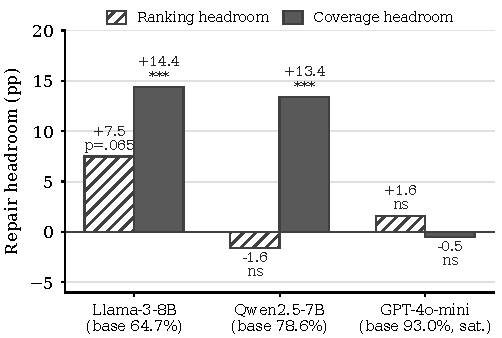
\includegraphics{figures/decomposition.pdf}
\caption{The decomposition of Table~\ref{tab:decomposition}: coverage
headroom (guaranteeing a perfect example exists) dwarfs ranking headroom
(perfectly selecting the best real example) on both non-saturated models and
vanishes on the saturated control. $^{***}$: $p{<}0.001$, exact McNemar.}
\label{fig:decomposition}
\end{figure}

\begin{table}
\caption{Coverage-vs-ranking decomposition ($n{=}187$; exact McNemar vs
baseline). Ranking headroom = \oraclecorpus $-$ base; coverage headroom =
planted $-$ \oraclecorpus.}
\label{tab:decomposition}
\begin{tabular}{lrrrr}
\toprule
Model (base) & \oraclecorpus & planted & rank.\ hr & cov.\ hr \\
\midrule
Llama-3-8B (64.7\%) & 72.2\% & 86.6\% & $+7.5$\rlap{$^{p=.065}$} & $\mathbf{+14.4}$\rlap{$^{***}$} \\
Qwen2.5-7B (78.6\%) & 77.0\% & 90.4\% & $-1.6$\rlap{$^{ns}$} & $\mathbf{+13.4}$\rlap{$^{***}$} \\
GPT-4o-mini (93.0\%) & 94.7\% & 94.1\% & $+1.6$\rlap{$^{ns}$} & $-0.5$\rlap{$^{ns}$} \\
\bottomrule
\end{tabular}
\end{table}

Table~\ref{tab:decomposition} and Figure~\ref{fig:decomposition} give the
central result. With a perfect example guaranteed present, repair jumps $+21.9\pp$ over baseline for
Llama-3-8B ($64.7\%{\to}86.6\%$, $p{<}0.0001$) and $+11.8\pp$ for Qwen2.5-7B
--- so retrieved examples \emph{can} convert failures when a sufficiently
relevant one exists. Decomposing that gain: \textbf{coverage headroom is
large and significant on both non-saturated models} ($+14.4$ and $+13.4\pp$)
and zero on the saturated control, while \textbf{ranking headroom is small
and heterogeneous} ($+7.5\pp$ marginal on Llama; $-1.6\pp$ on Qwen, where
even forcing the best real example does not help). We refuse to average the
two into a single ``ranking gap'': the honest claim is that the binding
constraint is \emph{primarily corpus coverage}, with inconsistent, at-best
marginal ranking headroom.

The most damaging finding for reranking sophistication: when the perfect
example is present, \emph{plain dense retrieval surfaces it in the top-$k$
100\% of the time}, while \structured reranking demotes it out of the top-$k$
in 11/187 cases (94.1\%) --- and repair conversion is identical for both
($86.6\%$). The relevance-proxy improvement of RQ1, even where it holds,
does not translate into better best-example selection; it slightly degrades
it. Relevance-to-repair conversion also fails at the instance level: among
the 37 problems where retrieval flips the 8B outcome (18 wins, 19 losses),
the mean retrieved-example relevance of wins ($2.645$) is indistinguishable
from losses ($2.621$).

For completeness, \oracleself\ (showing the model its own problem's exact
fix pattern) reaches $90.4\%$ ($+25.7\pp$, $p{<}0.0001$) on 8B --- a sanity
check that the model can exploit a near-identical example, not a deployable
ceiling.

\subsection{RQ4: Transfer to real repository bugs}
\label{sec:results-transfer}

Synthetic mutations make ``perfect examples'' constructible by design, so RQ3
could in principle be an artifact of the synthetic regime. We test transfer
on real PyBugHive \texttt{black} bugs end-to-end (environment build, patch
application through the line-range layer, full test suite).

With the project-held-out corpus (contamination-controlled), baseline,
\codeonly, and \structured all repair 23/34 --- retrieval is exactly neutral
on real bugs, consistent with RQ2. Planting the exact buggy$\to$fixed file
pairs into the corpus (34 plants + 551 filler) lifts GPT-4o-mini from
$85.7\%$ to $96.4\%$ on the 28 cleanly-paired cases, converting \emph{all
four} baseline failures while regressing one (McNemar $b{=}1$, $c{=}4$,
$p{=}0.375$). The patch layer did apply the planted fixes on large formatter
files, so the coverage effect is not blocked by repository-scale mechanics.

This transfer result is directionally positive but underpowered: black's high
baseline leaves only four failures to convert.
%% TODO(powered-CI): replace this paragraph with the powered result over 116
%% cases / 10 projects (pandas, jax, freqtrade, salt, spaCy, poetry, ...)
%% from the CI experiment; report pooled exact McNemar and per-project
%% breakdown, and update the abstract and Section 1 accordingly.
A powered replication over all 116 supported PyBugHive cases across 10
projects (executing in x86 containers to lift the local environment ceiling)
is in progress; we will report it in the final version.
